%%%%%%%%%%%%%%%%%%%%%%%%%%%%%%%%%%%%%%%%%%%%%%%%%%%%%%%%%%%%%%%%%
%  _____       ______   ____									%
% |_   _|     |  ____|/ ____|  Institute of Embedded Systems	%
%   | |  _ __ | |__  | (___    Wireless Group					%
%   | | | '_ \|  __|  \___ \   Zuercher Hochschule Winterthur	%
%  _| |_| | | | |____ ____) |  (University of Applied Sciences)	%
% |_____|_| |_|______|_____/   8401 Winterthur, Switzerland		%
%																%
%%%%%%%%%%%%%%%%%%%%%%%%%%%%%%%%%%%%%%%%%%%%%%%%%%%%%%%%%%%%%%%%%

\chapter{MIDI Steuerung}\label{chap.midi}

\section{Einteilen der Blöcke und definieren der Schnittstelen}

Als erstes die Zusammenfassung der internen Blöcke. Die zwei entwickelten Blöcke \textbf{midi control} und \textbf{polyphonie out} sind grau markiert (siehe Abbildung \ref{fig.midi_interface_block} ). Gegeben ist der Block uart top. \\

\begin{figure}[H]
	\centering
	\includegraphics[width=1\textwidth]{images/midi_interface/midi_interface_block.png}
	\caption{Blockschaltbild MIDI Interface}
	\label{fig.midi_interface_block}
\end{figure}

Die Abbildung \ref{fig.top_synthesizer_block} (im Anhang \ref{chap.anhang_top_synthesizer}) zeigt, wie das zu entwickelnde MIDI Interface in die bestehenden Blöcke des Synthesizer-Projektes eingebaut wird. Die im Anhang direkt anschliessende Abbildung \ref{fig.top_synthesizer_detail} zeigt dann die geplante Umsetzung detaillierter.\\




Als nächstes wird die MIDI 1.0 Spezifikation, erklärt, nach der Block \textit{midi control} aufgebaut ist. Die Umsetzung des \textit{polyphone out}-Blocks bildet den Abschluss dieses Kapitels.\\


\newpage
\section{Das MIDI Kommunikationsprotokoll}\label{sect.midi_spezification}
Werden MIDI Daten übermittelt, so unterscheidet der Standard zwei Typen an Daten \ref{Midi_specification}.

\subsection{MIDI Daten Typen}\label{datenytpen}
\subsubsection*{Status Bytes}
\textit{Status bytes} sind 8 Bit lang und das MSB ist immer logisch '1'. Die \textit{status bytes} dienen dem Identifizerein der nachfolgenden \textit{data bytes}. Das \textit{status byte} sagt, von welcher Art und mit welcher Datenstruktur die folgenden \textit{data bytes} sein werden.
\newline
\newline
MIDI behält einen Status so lange, bis ein neues \textit{status byte} folgt. Dieses Verhalten wird als \textit{running status} bezeichnet. Dieses Verhalten ist vor allem für die Polyphonie interessant, da dieser Zustand bleibt und viele \textit{Data Bytes} (im Sinn von Noten) folgen können, ohne dass es eines neuen status bytes bedarf.

\subsubsection*{Data Bytes}
Gemäss Spezifikation folgen einem \textit{status byte} exakt ein oder zwei Bytes. Das MSB ist immer logisch '0'. Die Werte können von 0x00 bis 0x7F sein. Das bedeutet, dass MIDI maximal 128 Noten unterscheiden kann.
\newline
\newline
\textit{Data bytes} können unterschiedliche Informationen erhalten. Im Kontroller sind Notenwerte, Geschwindigkeit des Anschalges releant
\newline
\newline
Je nachdem welches \textit{status byte} im Voraus gesetzt wurde, werden die Attribute anders interpretiert.Ist z.B. Polyphonie gesetzt, so bedeutet ein \textit{data byte} mit einer Geschwindigkeit von 0, Note abstellen. Diese und andere Spezifikationen werden detailliert in \textbf{Detailierte Spezifikation} beschrieben.
\newline
\newline
''Empfänger sollen so konzipiert sein, dass zuerst alle\textit{data bytes} empfangen werden und ein neues \textit{status byte} kommt. Danach werden ungültige Daten verworfen. Einzige Ausnahme ist der \textit{running status}. Bei dem nicht bis zum Ende gewartet wird.''\ref{Midi_specification}.\\

\subsubsection*{Ungültige Bytes}
''Alle \textit{status bytes}, die nicht implementierte Funktionen enthalten und alle ihnen folgenden \textit{Data Byte}s sollen vom Empfänger verworfen werden.''\ref{Midi_specification}.\\ MIDI Geräte sollen ausdrücklich beim Ein- und Abstellen darauf bedacht sein, dass keine undefinierten Bytes gesendet werden\ref{Midi_specification}.\\
Diese Anforderung ist wichtig beim Implementieren der \textit{finate state machine} und der \textit{testbench} (siehe \ref{polyphonitest}) \\

\subsection{Zwei MIDI Note Modes}\label{note_modes}
\subsubsection{single mode}
\begin{figure}[H]
	\centering
	\includegraphics[width=1\textwidth]{images/midi_interface/MIDI_Spezifikation.png}
	\caption{Blockschaltbild Device under Test}
	\label{fig.testbench_single_Mode}
\end{figure}

Im Fall der einzelnen Note passt die Tokenstruktur, die sich am schwierigsten Fall, der Polyphonie orientierte, nicht ganz. Im Gegensatz zur Polyphonie muss bei der einzlenen Note VOR dem Notenwert ein status byte kommen. Damit dies in der Tokenstruktur umsetzbar ist, wird zuerst ein Dummy-Wert (55) zum Verwerfen der \textit{testbench} übergeben. Erst dann folgt das \textit{status byte} und dann, analog zur Polyphony-Sturktur folgt die erste Note. Im Nachhinein erscheint mir dieser Aufbau als zu kompliziert und ich würde ein nächstes Mal mehr mode-spezifisch die Datenauswertung gestalten.


\subsubsection{polyphony mode}
\begin{figure}[H]
	\centering
	\includegraphics[width=1\textwidth]{images/midi_interface/MIDI_Spezifikation_Datenfolge.png}
	\caption{Blockschaltbild Device under Test}
	\label{fig.testbench_polypphon_mode}
\end{figure}
Danach werden die Token gemäss der Polyphonie-Spezifikation interpretiert: Die \textit{data bytes} wechseln sich ständig mit dem Notenwert und der dazugehörenden Geschwindigkeit ab. Hier in der Testdatei hält die erste Note den Wert 71 und wird gefolgt von irgendeiner Geschwindigkeit (hier Dummy-Wert 55), usw.. Kommt ein Geschwindigkeitswert von 0, so bedeutet dies, dass die Note abgestellt wird.
Danach werden die Token gemäss der Polyphonie-Spezifikation interpretiert: Die \textit{data bytes} wechseln sich ständig mit dem Notenwert und der dazugehörenden Geschwindigkeit ab. 

\section{Umsetzung "midi control"-Block}\label{sect.midi_umsetzung}
Ausgehend von der Spezifikation sind drei Eckpunkte für die \textit{finite state machine} zu berücksichtigen:\\
\begin{enumerate}
	\item Unterscheiden von \textit{status byte} und \textit{data byte}
	\item Unterschiedliche Interpretation der \textit{data bytes} abhängig vom \textit{status byte}.
	\item Verwerfen aller falschen \textit{status byte} oder \textit{data bytes}
\end{enumerate}

Zu beachten in der Verarbeitung der Daten ist, dass im \textit{single mode} zuerst gesagt wird, ob eine Note an oder ab und diese Reihenfolge im \textit{polyphony mode} gerade umgekehrt ist: zuerst kommt die Note, dann die Angabe, ob sie an oder ab ist.

Aus diesen Anforderungen ergab sich folgende \textit{finite state machine}:

\begin{figure}[H]
	\centering
	\includegraphics[width=1\textwidth]{images/midi_control/fsm_midicontrol.png}
	\caption{fsm Übergänge}
	\label{fig.midi_fsm_inksape}
\end{figure}
Alle drei Anforderungen sind implementiert:\\
Vor jedem \textit{data byte} muss zuerst ein \textit{status byte} eingegangen sein. Die \textit{finite state machine} fragt im \textit{idle} Zustand nur nach den \textit{status bytes}. So weisen die oberen Nibbel mit den Werten "1001" für NOTE AN und "1000" für NOTE AUS auf den  \textit{single mode} hin und der Wert "1010" auf den \textit{polyphony mode}. Nach diesen \textit{status bytes} erwartet die \textit{finate state machine} \textit{data bytes}.\\ 
Die unterschiedliche Reihenfolge von Noten-Byte und Angaben zu an oder ab, wurde statusabhängig umgesetzt:\\
%fig.midi_fsm_inksape
%(siehe Abbildung fig.midi_fsm_inksape )
Im \textit{single mode} wird das vierte Bit des \textit{status nibbel} zum Setzen von AN und AB verwendet . Im polyphony mode wird das zweite \textit{data byte}, das ueblicherweise die Geschwindigkeit der Note bestimmt, für das Setzen von AN und AUS genommen. Ist der Wert der Geschwindigkeit gleich NULL, dann soll in diesem Zustand die Note als AUS gelten.\\
Gut sichtbar ist, dass die \textit{finite state machine} bei ungültigen \textit{bytes}, die Daten verwirft und in den \textit{idle} Zustand zurückgeht.\\

\begin{figure}[H]
	\centering
	\includegraphics[width=1\textwidth]{images/midi_control/fsm_midi_control_inkskape.png}
	\caption{fsm Übergangsbedingungen}
	\label{fig.midi_fsm_quartus}
\end{figure}

Das Umsetzung der \textit{fsm} sieht man in der simulation in den zweit unteren Abbildungen gut. Nach dem Zustand \textit{idle} folgt das \textit{status byte} "single" (Abbildung \ref{fig.midicontrol_singlet} )oder "polyphonie" (Abbildung \ref{fig.midicontrol_polyphonie} )\\  

\begin{figure}[H]
	\centering
	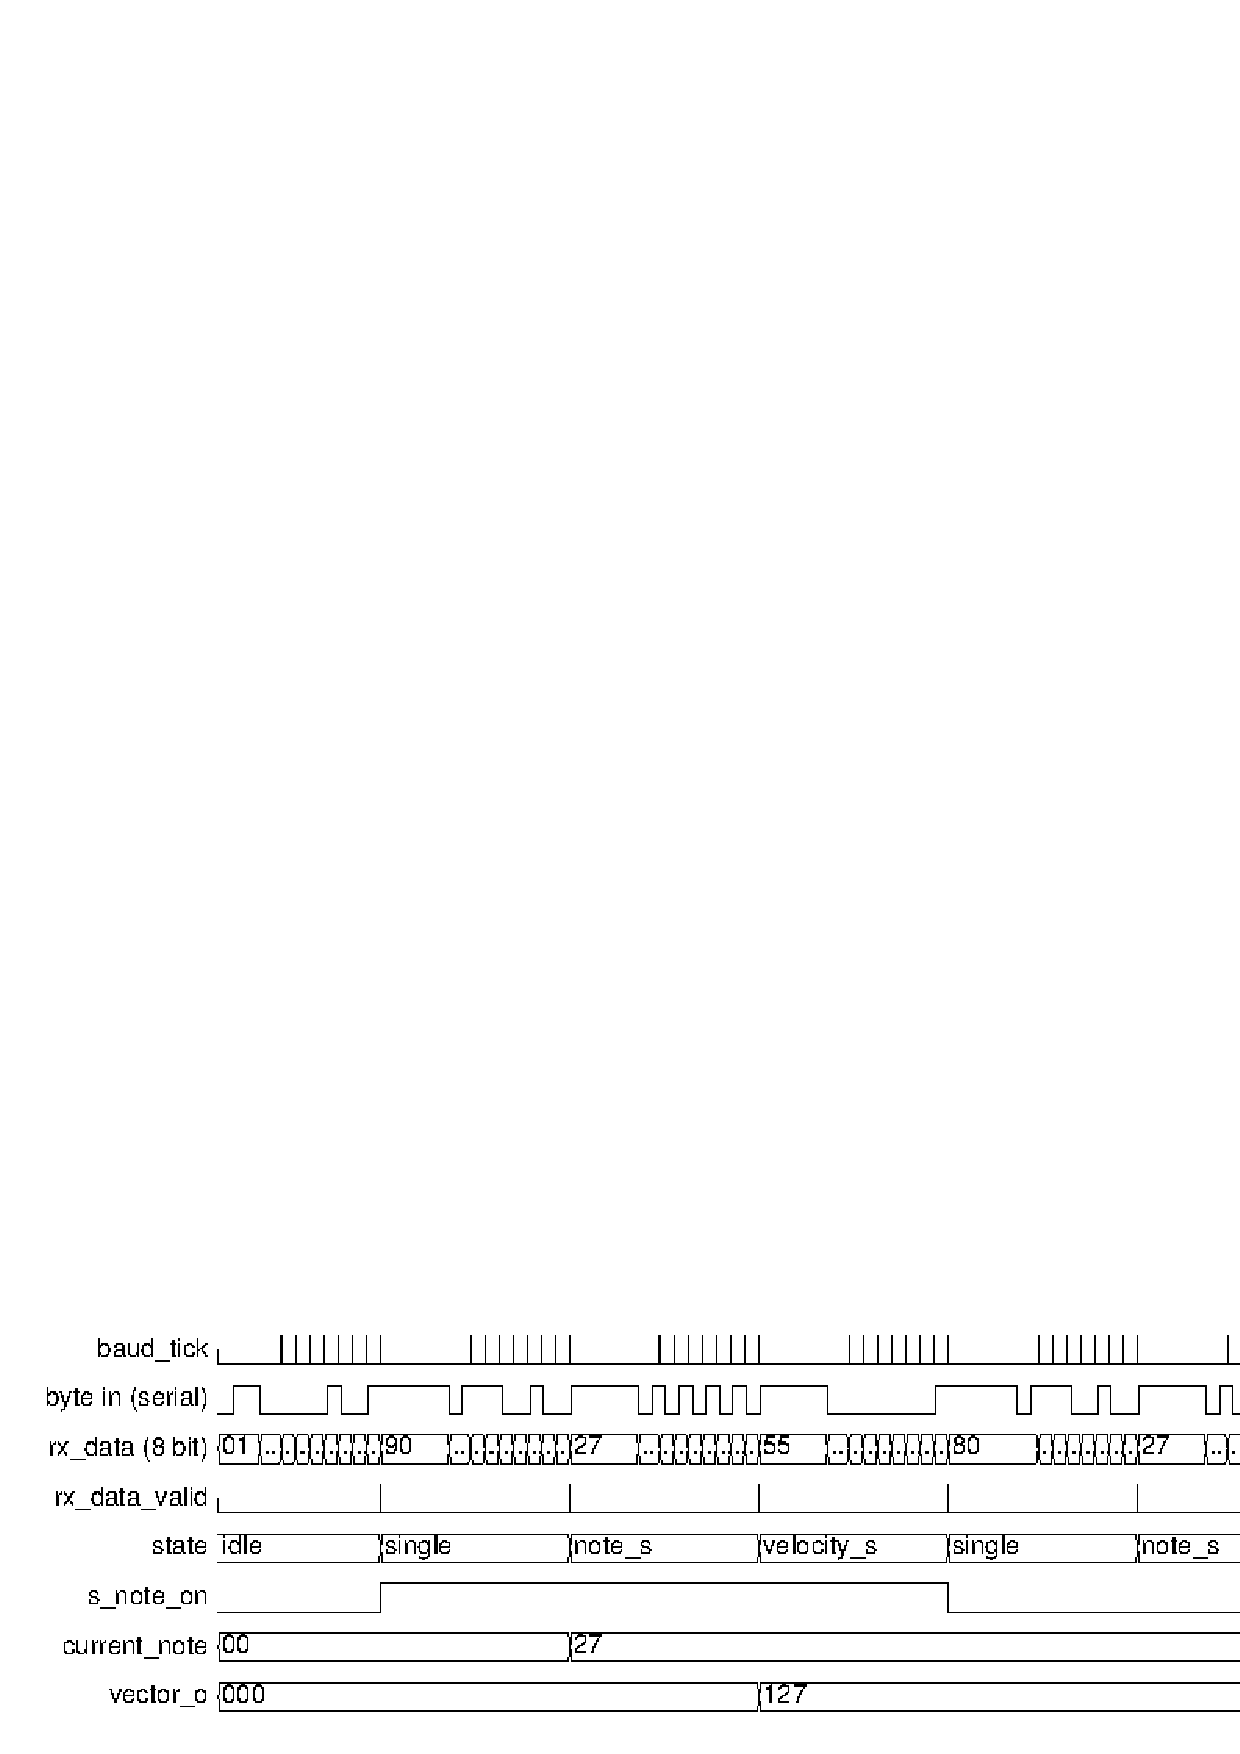
\includegraphics[width=1\textwidth]{images/midi_control/wave_single.png}
	\caption{fsm für single mode}
	\label{fig.midicontrol_singlet}
\end{figure}

\begin{figure}[H]
	\centering
	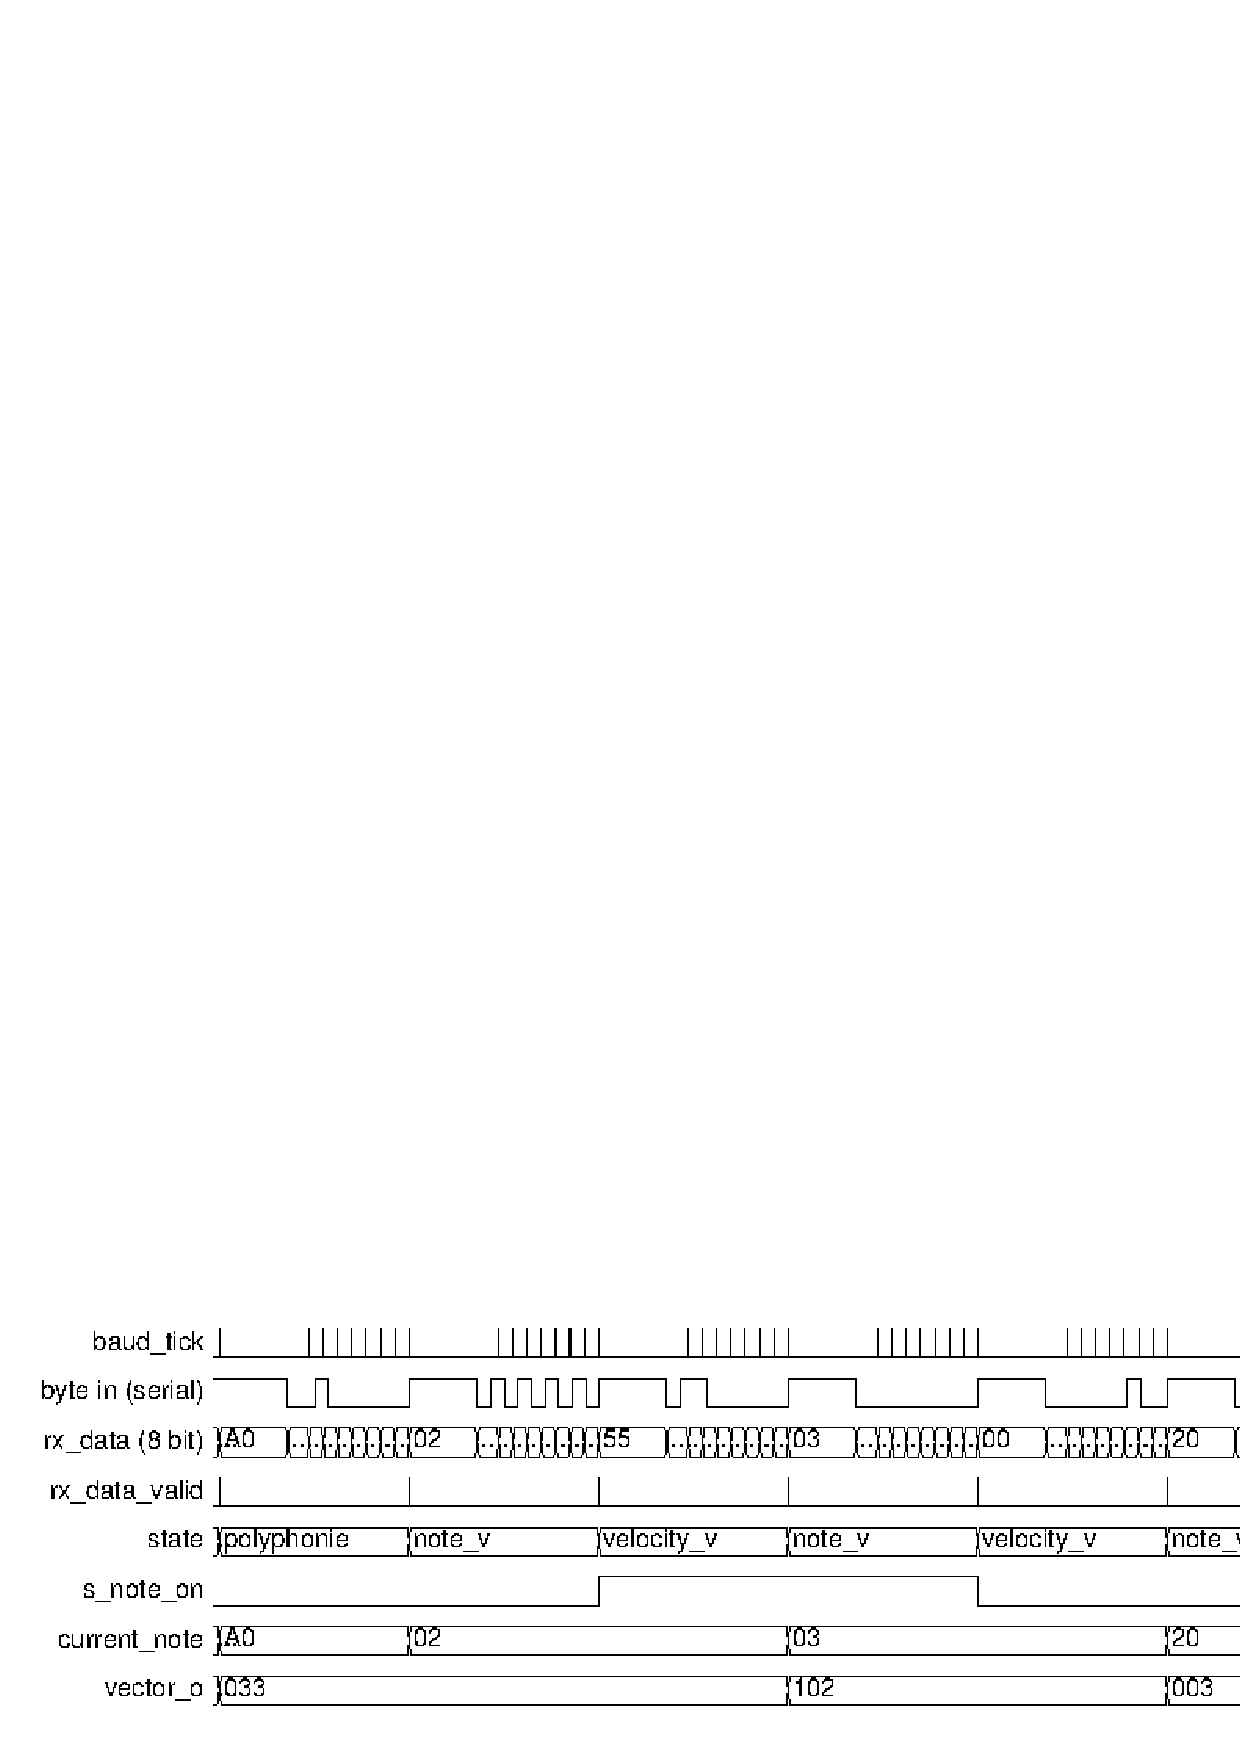
\includegraphics[width=1\textwidth]{images/midi_control/wave_polyphonie.png}
	\caption{fsm im polyphony mode}
	\label{fig.midicontrol_polyphonie}
\end{figure}

Die Simulation wurde mit möglichen Fehlübertragungen angereichert, damit man sieht, ob der \textit{midi control} weiter korrekt funktionert. Eine detaillierte Beschreibung zum Aufbau der Simulation befindet sich im Kapitel \textbf{testbench}.\\


\section{Umsetzung "polyphonie out"-Block}\label{sect.polyphonie_umsetzung}